
\documentclass[12pt]{article}

\newcommand{\VERSION}{1.8.0}

\usepackage[utf8]{inputenc}
\usepackage[english]{babel}
\usepackage{csquotes}

\usepackage{xcolor}
\usepackage{listings, lstautogobble}

\usepackage{booktabs}
\setlength{\heavyrulewidth}{1.5pt}
\setlength{\abovetopsep}{4pt}

\lstset{language=bash,
	keywordstyle=\color{black},
	basicstyle=\small\ttfamily,
	commentstyle=\ttfamily\itshape\color{gray},
	stringstyle=\ttfamily,
	showstringspaces=false,
	breaklines=true,
	frameround=ffff,
	frame=single,
	rulecolor=\color{black},
	autogobble=true
}

\usepackage{hyperref}
\hypersetup{
	colorlinks=true,
	linktoc=all,
	linkcolor=blue,
	citecolor=blue
}

\begin{document}
	
	\title{DTarray\_pro-\VERSION \space User Guide}
	\author{Aaron Maurais}
	\date{14 June 2019}
	
	\maketitle
	\tableofcontents
	\newpage
		
	\section{Introduction}
	
	\texttt{DTarray\_pro} extracts Uniprot ID numbers, molecular weights, and spectral counts from DTASelect-filter files. Protein data is combined into one dataset and written to the working directory as a tab delimitated text file (.tsv). This document will describe how to install and use the latest version of \texttt{DTarray\_pro} step by step. Some experience using a unix shell is assumed.  
	
	
	\section{Installation}
	
	\subsection{Downloading DTarray\_pro source code.}

	\begin{itemize}

	\item \texttt{DTarray\_pro} expects to be installed in \texttt{\$HOME/local}. The program needs files stored in \texttt{\$HOME/local/DTarray\_pro/db} for some features to work. First, make \texttt{\$HOME/local} if it doesn't exist.

	\begin{lstlisting}
	 		$ mkdir -p ~/local
	\end{lstlisting}

	\item If you do not wish to build the program in \texttt{\$HOME/local}, you can run the configure script from the desired location with the \texttt{--program-directory <path>} option.

	\item \texttt{DTarray\_pro} is hosted at GitHub, which is a free hosting service for distributed version control in software development. To clone the latest version of the stable branch from the GitHub repo into your current working directory, run:

	\begin{lstlisting}
		$ git clone --recurse-submodules --single-branch --branch stable https://github.com/ajmaurais/DTarray_pro
	\end{lstlisting}

	\end{itemize}

	\subsection{Compiling DTarray\_pro}

	\begin{itemize}

	\item \texttt{DTarray\_pro} is written in vanilla c++ 11 and can be compiled on linux or macOS systems with gcc. Other compilers may work but have not been tested.

	\item To configure and build \texttt{DTarray\_pro}, run:

	\begin{lstlisting}
		$ cd ~local/DTarray_pro
		$ ./configure
		$ make
	\end{lstlisting}

	\item After you have run \texttt{make}, there should be several new files in the \texttt{DTarray\_pro} directory.  If everything worked, two executable files should be located at \texttt{DTarray\_pro/bin/}
		
	\begin{lstlisting}
		$ ls bin
		DTarray		DTsetup
	\end{lstlisting}
		
	\item \texttt{DTarray} is the executable for \texttt{DTarray\_pro}
		
	\item \texttt{DTsetup} is the executable for a script which will automatically setup DTASelect-filter to be read into \texttt{DTarray\_pro}.

	\end{itemize}

	% \subsection{Installing DTarray\_pro and DTsetup (optional)}


	
	% To run \texttt{DTarray\_pro} you have to navigate on your terminal to a folder which contains DTASelect-filter files then type the full path to the executable file.  Its possible to install a program system wide so you don't have to type the path every time, but without administrative privileges, its a bit complicated. A workaround is to create a shortcut or alias to the executable file.  This section will explain how to add an alias for \texttt{DTarray\_pro} and \texttt{DTsetup} to your shell profile on \texttt{pleiades}
	
	% \begin{itemize}
	% 	\item To add an alias for \texttt{DTarray\_pro} and \texttt{DTsetup}, you will have to edit your shell profile, which is a file stored in your home directory named \texttt{.tcshrc}.
		
	% 	\item To edit your shell profile, you will use a command line text editor called \texttt{nano}. To open \texttt{.tcshrc} in \texttt{nano}, type:
		
	% 	\begin{lstlisting}
	% 		$ cd
	% 		$ nano .tcshrc
	% 	\end{lstlisting}
		
	% 	\item After starting \texttt{nano}, your terminal window should look something Figure \ref{fig:step_1}.
		
	% 	\begin{figure}[h!]
	% 		\centering
	% 		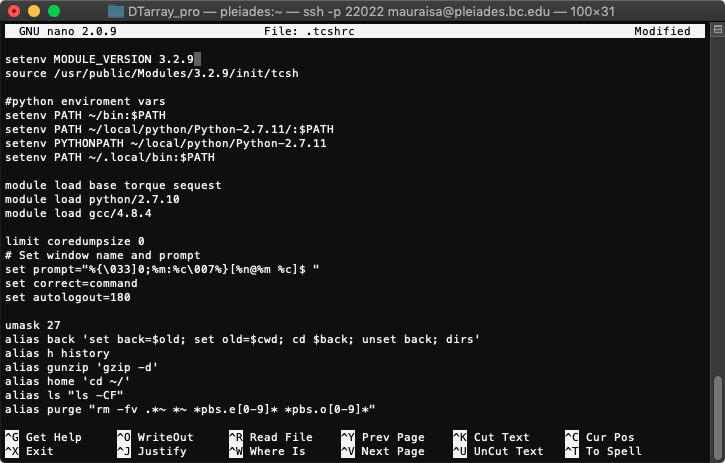
\includegraphics[width=0.7\textwidth]{step_1.png}
	% 		\caption{Example terminal window after opening \texttt{.tcshrc} with \texttt{nano}}
	% 		\label{fig:step_1}
	% 	\end{figure}
		
	% 	\item Scroll to the bottom of the file and add the lines: \\
	% 	\texttt{alias DTarray "\textasciitilde/local/DTarray\_pro-\VERSION/bin/DTarray"} \\
	% 	\texttt{alias DTsetup "\textasciitilde/local/DTarray\_pro-\VERSION/bin/DTsetup"} \\
	% 	(See Figure \ref{fig:step_2} for an example).
		
	% 	\begin{figure}[h!]
	% 		\centering
	% 		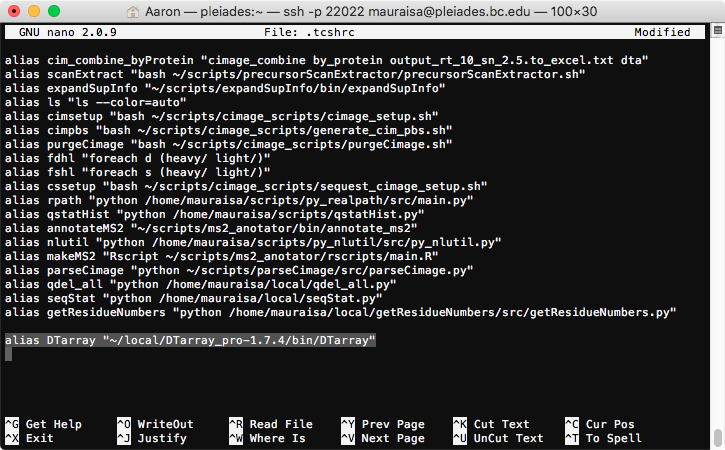
\includegraphics[width=0.7\textwidth]{step_2.png}
	% 		\caption{\texttt{.tcshrc} with new aliases for \texttt{DTarray\_pro} and \texttt{DTsetup}}
	% 		\label{fig:step_2}
	% 	\end{figure}
	
	% 	\item To save and exit the file, hit \texttt{\textasciicircum + X}. A dialog should show up at the bottom which says: 
	% 	\begin{lstlisting}
	% 		Save modified buffer (ANSWERING "No" WILL DESTROY CHANGES) ?
	% 	\end{lstlisting}
	% 	\item Hit \texttt{y}
		
	% 	\item Next a dialog should show up at the bottom which says 
		
	% 	\begin{lstlisting}
	% 		File name to write: .tcshrc
	% 	\end{lstlisting}
		
	% 	\item Hit \texttt{enter} to exit.
		
	% 	\item Finally you have to tell the computer to reload your shell profile after you have modified it with the command:
		
	% 	\begin{lstlisting}
	% 		$ source .tcshrc
	% 	\end{lstlisting}
		
	% 	\item You can test your alias by typing the following command from your home directory:
		
	% 	\begin{lstlisting}
	% 		$ DTarray --version
	% 	\end{lstlisting}
		
	% 	\item If the alias is recognized by the computer, it should display something like:
		
	% 	\begin{lstlisting}
	% 		DTarray_pro 1.7
	% 		Last git commit: Sat Sep 22 20:28:17 2018
	% 		git revision: 04d30f4fd7790abfca60197d85cefc9d2a
	% 	\end{lstlisting}
		
	% \end{itemize}
	
	
	\section{Usage}
	
	\subsection{Setting up filter files with DTsetup} \label{sec:dtsetup}
	
	\texttt{DTsetup} searches all directories one level below where it is run for a file named \texttt{DTASelect-filter.txt}. If a matching file is found, it is copied into a folder named \texttt{<date>\_<time>\_dtarraySetup} with the name \texttt{<sample\_name>.dtafilter}. Once \texttt{DTsetup} is run, \texttt{DTarray\_pro} can be run from the newly created directory to compare spectral counts for proteins found in multiple runs.
	
	\bigskip
	\noindent
	To run \texttt{DTsetup}, first navigate to a directory containing subdirectories with \texttt{DTASelect-filter.txt} files and run the command:
	
	\begin{lstlisting}
		$ DTsetup
		Creating dtarraySetup folder in parent dirrectory...
		Copying DTA filter files to 18-09-28_121625_dtarraySetup
			Adding ./sample_1...
			Adding ./sample_2...
			Adding ./sample_3...
			Adding ./sample_4...
		Done
	\end{lstlisting}
	
	\subsection{DTarray\_pro Input format options}
	
	Users have two options for how the input DTASelect-filter files read in by \texttt{DTarray\_pro} are structured.  
	
	\subsubsection{std mode} 
		
	In \texttt{std} mode, DTASelect-filter are stored in a common directory and the files are named with the format \texttt{<sample\_name>.dtafilter} (This is the default input mode for \texttt{DTarray\_pro}.)
	
	\begin{lstlisting}
		$ ls
		sample_1.dtafilter		sample_2.dtafilter
		sample_3.dtafilter		sample_4.dtafilter
	\end{lstlisting}
	
	\noindent
	The user can either manually setup the folder, or use \texttt{DTsetup} to automatically generate the folder.  To run \texttt{DTarray\_pro} in \texttt{std} mode, run the commands:
	
	\begin{lstlisting}
		$ cd <path_to_directory_with_filterfiles>
		$ DTarray
		
		DTarray_pro v1.7
		
		Adding sample_1...
		Adding sample_2...
		Adding sample_3...
		Adding sample_4...
		
		4 files combined.
		
		Writing protein data... done!
		Protein data written in wide format to: DTarray_pro.tsv
		
	\end{lstlisting}
	
	\noindent
	If \texttt{DTarray\_pro} was successful, two files should have been generated.  \texttt{DTarray\_pro.tsv} is a tab delimitated text file (.tsv) which contains a row for each protein and a column for the spectral counts of that protein in each sample.  \texttt{dtarray\_pro\_flist.txt} is a list of valid \texttt{.dtafilter} files found in the directory.  If a file list already exists in the folder, the existing file list is used.  The user can edit the file list to change the order of the columns in the output file and add additional files to the list.  
	
	\pagebreak
	\subsubsection{subidr mode}
	
	In \texttt{subdir} mode, DTASelect-filter files are stored in a separate directory, the directory name is the sample name, and the filter files are named \texttt{DTASelect-filter.txt} (This is the default input mode for \texttt{dtarray.pl}.)
	
	\begin{lstlisting}
		$ find */*.txt
		sample_1/DTASelect-filter.txt
		sample_2/DTASelect-filter.txt
		sample_3/DTASelect-filter.txt
		sample_4/DTASelect-filter.txt
	\end{lstlisting}
	
	\noindent
	To run \texttt{DTarray\_pro} in \texttt{subdir} mode, the user has to include the \texttt{-i subdir} option, because \texttt{subdir} is not the default behavior.  
	
	\begin{lstlisting}
		$ cd <path_to_parent_directory>
		$ DTarray -i subdir
	\end{lstlisting}
	
	\noindent
	Upon completion, a files named \texttt{DTarray\_pro.tsv} and \texttt{dtarray\_pro\_flist.txt} are generated formatted the same as in \texttt{std} mode.
	
	\subsection{DTarray\_pro Output file options}
	
	This document will not provide an exhaustive list of options for \texttt{DTarray\_pro}. Instead, this section will provide examples of options will likely find most useful.  For the full list of optional arguments see \texttt{DTarray\_pro/helpFile.pdf} or use \texttt{DTarray -h} to see the help file from the terminal.
	
	\subsubsection{Get spectral counts for unique peptides by protein} \label{sec:unique_sc}
	
	the \texttt{-u} option is used to include a column for the total counts for unique peptides in the \texttt{DTarray\_pro.tsv} output file.
	
	\begin{lstlisting}
		$ DTarray -u
	\end{lstlisting}
	
	By default, the columns for spectral counts and unique peptide spectral counts are grouped by sample.  See section \ref{sec:sup_info} to change this behavior.  
	
	\subsubsection{Specify how to group supplementary information columns in output file} \label{sec:sup_info}
	
	The examples in this section all use the \texttt{-u} option (section \ref{sec:unique_sc}), but the \texttt{-s} option is also compatible with other \texttt{DTarray\_pro} options including the \texttt{-lr} option (see section \ref{sec:loc})
	
	\bigskip
	\noindent
	By default, the columns for sample specific supplementary information are grouped by sample as shown in table \ref{table:s_0}.  
	
	\bigskip
	\begin{table}[h!]
		\centering
		\footnotesize
		\begin{tabular}{ccccc}
			\toprule
			& \multicolumn{2}{c}{Sample\_1}
			& \multicolumn{2}{c}{Sample\_2} \\
			\midrule
			Protein & SC & Unique\_SC & SC & Unique\_SC \\ 
			\midrule
			ALBU & 2149 & 2149 & 3092 & 3092 \\
			TRFE & 661 & 661 & 698 & 698 \\ 
			IGHG1 & 573 & 152 & 382 & 52 \\ 
			\toprule
		\end{tabular}
		\caption{Default column arrangement}
		\label{table:s_0}
	\end{table}
	
	%\bigskip
	\noindent
	The \texttt{-s} option can be used to control this behavior. To group the columns by sample , then observation (table \ref{table:s_1}) add the \texttt{-s 1} option.
	
	\begin{lstlisting}
		$ DTarray -u -s 1
	\end{lstlisting}
	
	\begin{table}[h!]
		\centering
		\footnotesize
		\begin{tabular}{ccccc}
			\toprule
			& \multicolumn{2}{c}{SC}
			& \multicolumn{2}{c}{Unique\_SC} \\
			\midrule
			Protein & Sample\_1 & Sample\_2 & Sample\_1 & Sample\_2 \\ 
			\midrule
			ALBU & 2149 & 3092 & 2149 & 3092 \\
			TRFE & 661 & 698 & 661 & 698 \\ 
			IGHG1 & 573 & 382 & 152 & 52 \\ 
			\toprule
		\end{tabular}
		\caption{Grouping columns by sample}
		\label{table:s_1}
	\end{table}
	
	\subsubsection{Get spectral counts for peptides}
	
	\noindent
	By default no peptide file is generated.  To also generate a file containing spectral counts for peptides in each sample, use the \texttt{-p 1} option.
	
	\begin{lstlisting}
		$ DTarray -p 1
	\end{lstlisting}
	
	\noindent
	An additional file will be generated named \texttt{peptideList.tsv} containing peptide data.
	
	\subsubsection{Modify how peptides are grouped in output file}
	
	\noindent
	By default, peptides are grouped by sequence and parent protein.  A separate entry for each	charge state of a given peptide will be  included  in  peptide	output files.  If the \texttt{-g 2} option is set, peptides will also be grouped by charge; i.e., the spectral counts for each peptide will be the sum of all charge states identified for that peptide.
	
	\begin{lstlisting}
		$ DTarray -p 1 -g 2
	\end{lstlisting}
	
	\noindent
	The \texttt{-modG <group\_method>} specifies how to group modified peptides in \texttt{peptideList.tsv}.  By default peptides  with  the  same sequence, but different modification status will not be grouped. A separate entry will be  included for each modification status found for a peptide. To ignore modification status when grouping peptides, use the \texttt{-modG 1} option.
	
	\begin{lstlisting}
		$ DTarray -p 1 -modG 1
	\end{lstlisting}
	
	\noindent
	If the \texttt{-p 1} option is not set, the \texttt{-g} and \texttt{-modG} will be ignored. The \texttt{-g} and \texttt{-modG} options can also be combined as desired.  
	
	\subsubsection{Get subcelluar location data for proteins} \label{sec:loc}
	
	\texttt{DTarray\_pro} can use \texttt{DTarray\_pro/db/humanLoc.tsv}  to lookup subcelluar localization information for proteins.  \texttt{humanLoc.tsv} contains Uniprot annotations for subcelluar localization by Uniprot ID,	updated as of Apr 19, 2019. Currently, sub cell location information is available for human proteins only.
	
	\bigskip
	\noindent
	There are two ways in which subcelluar location information can be compiled.
	
	\begin{enumerate}
		\item The \texttt{-loc} option will add a column for the location of each protein in \texttt{DTarray\_pro.tsv}.  To include the subcelluar location column in \texttt{DTarray\_pro.tsv} run the command:
		
		\begin{lstlisting}
			$ DTarray -loc
		\end{lstlisting}

		\item The \texttt{-lr 1} option will create a file named \texttt{loc\_summary.tsv} with the sum of spectral counts, sequences, and proteins identified for each subcelluar location.  To generate \texttt{loc\_summary.tsv} run the command:
		
		\begin{lstlisting}
			$ DTarray -lr 1
		\end{lstlisting}
		
		\noindent
		By default, columns are arranged by sample.  The \texttt{-s 1} option can be used to arrange the columns by observation.  See section \ref{sec:sup_info} for an explanation of the \texttt{-s} option.  
	
	\end{enumerate}
	
	\subsubsection{Calculate molecular weights for peptides and proteins}
	
	\texttt{DTarray\_pro} will calculate protein/peptide molecular weights and  molecular  formulas when the \texttt{-mw} option is provided. Columns  will  be  included in output files for average mass, monoisotopic mass and molecular formula.  
	
	%\pagebreak
	\bigskip
	\noindent
	Three files are required for the calculation:
	
	\begin{enumerate}
		\item  An atom count table, named \texttt{atomCountTable.txt} which contains the number and types of atoms found in each amino acid (similar to \texttt{Cimage} table).
		
		\item An atom mass table, located at \texttt{DTarray\_pro/db/atomMasses.txt}, containing the masses of each atom.  
		
		\item A \texttt{.fasta} file to lookup protein sequences located at \\ \texttt{DTarray\_pro/db/humanProteome.fasta} (required for proteins only) Currently, the \texttt{-mw} option is supported for human proteins only.
	\end{enumerate}
	
	\noindent
	By default the atom count table located at \texttt{DTarray\_pro/db/atomCountTable.txt} is used. The default atom count table includes a static modification on cysteine for iodoacetamide alkylation.  To calculate peptide and protein masses with default residue masses, run:
	
	\begin{lstlisting}
		$ DTarray -p 1 -mw
	\end{lstlisting}
	
	\noindent
	The  user  can  also supply a custom \texttt{atomCountTable.txt} file with the \texttt{-act <file\_name>} option. A copy of the default atom count table can be generated in the working directory with the \texttt{-mact} option.  
	
	\begin{lstlisting}
		# make default atomCountTable.txt in working directory
		$ DTarray -mact
		# run DTarray with custom atomCountTable.txt
		$ DTarray -act ./atomCountTable.txt -p 1 -mw
	\end{lstlisting}
	
	\noindent
	The user can also edit the default atom count table as at \\ \texttt{DTarray\_pro/db/atomCountTable.txt} as desired, but editing \\ \texttt{DTarray\_pro/db/atomMasses.txt} is not recommended.
	
\end{document}
